\section{Grouping objects}


\subsection{Selfstudy-Questions OOP5}

\subsubsection{Chapter 4.1 to 4.3 - An organizer for music files}

\subsubsection*{Exercise 1}
\textit{Solve the exercises 4.1 to 4.3}\\

\textbf{4.1}

\lstinputlisting{../workspace/Music-Organiser-V1/src/music/MusicOrganizer.java}
\lstinputlisting{../workspace/Music-Organiser-V1/src/music/Main.java}

\textbf{4.2} We don't get an error. As wee look at the code of the method
we'll see, that the method is examinating if the index is "valid". If not
it does not perform a remove action.

\lstinputlisting[firstline=58, lastline=63]{../workspace/Music-Organiser-V1/src/music/MusicOrganizer.java}

\textbf{4.3} The list is shifted, so that the previously second track is the
first track after removing the first track.

\subsubsection*{Exercise 2}
\textit{What do you understand by "Java-Package"?}\\

A Java-Package is just a collection of classes. It is a namespace to organize
classes.

\subsubsection*{Exercise 3}
\textit{You want to use the library-class ArrayList. What expression makes it
possible to use that library-class in your source code?}\\

\noindent
If we want to use a library-class, we have to import it to our source with

\lstinline{import java.nameOfTheLibraryClass;} \\

\noindent
So to use the ArrayList we just have to write in our source 

\lstinline{import java.util.ArrayList;} 

\subsubsection{Chapter 4.4 to 4.7 - Numbering within collections}

\subsubsection*{Exercise 4}
\textit{Solve the exercises 4.4 to 4.7}\\

\subsubsection*{Exercise 4.4, page 100}  
\textit{Write a declaration of a private field named library that can hold an
ArrayList. The elements of the ArrayList are of type Book.}\\

\lstinline{private ArrayList<Book> library = new ArrayList<String>();}

\subsubsection*{Exercise 4.5, page 100}
\textit{Write a declaration of a local variable called cs101 that can hold an
ArrayList of Student.}\\

\lstinline{private ArrayList<Student> cs101 = new ArrayList<Student>();}

I'm not really sure about the "local" in the exercise. Do I have to specify
that this is private or not?

\subsubsection*{Exercise 4.6, page 101}
\textit{Write a declaration of a private field called tracks for sorting
a collection of MusicTrack objects.}\\

\lstinline{private ArrayList<MusicTrack> tracks = new ArrayList<MusicTrack>();}

\subsubsection*{Exercise 4.7, page 101}
\textit{Write assignments to the library, cs101 and track variables (which
you defined in the previous three exercises) to create the appropriate 
ArrayList objects. Write them once without using diamond and once with
diamond notation if you are using Java 7 compiler.}\\

\begin{lstlisting}
library.add("Objects First with Java");
cs101.add("Leonardo DaVinci");
track.add("Free Software Song");
\end{lstlisting}

I'm not really sure what is the question here \dots

\subsubsection*{Exercise 5}
\textit{Solve the exercises 4.8 to 4.11}\\

\subsubsection*{Exercise 4.8, page 102}
\textit{If a collection stores 10 objects, what value would be returned from
a call to its size method?}\\

It would return 9.

\subsubsection*{Exercise 4.9, page 102}
\textit{Write a method call using get to return the fifth object stored in a
collection called items.}\\

\lstinline{items.get(4)}

\subsubsection*{Exercise 4.10, page 102}
\textit{What is the index of the last item stored in a collection of 15
objects?}\\

This would be 14.

\subsubsection*{Exercise 4.11, page 102}
\textit{Write a method call to add the object held in the variable 
favoriteTrack to a collection called files.}\\

\lstinline{addFavorite(favoriteTrack, files)}

I'm not really sure about this question \dots

\subsubsection*{Exercise 6}
\textit{Solve the exercises 4.12 to 4.13}\\

\subsubsection*{Exercise 4.12, page 103}
\textit{Write a method call to remove the third object stored in a
collection called dates.}\\

\lstinline{dates.remove(2)}

\subsubsection*{Exercise 4.13, page 103}
\textit{Suppose that an object is stored at index 6 in a collection.
What will be its index immediately after the objects at index 0 and 9
are removed?}\\

After removing index 0, the whole collection is shifted by $-1$, 
so the index of the element, which was at index 5 in the beginning
would now be at $6-1=5$. Removing an index after the queried one has
non effect of the indexing, so it would still be 5.

\subsubsection*{Exercise 7}
\textit{Explain the following declaration:}\\
\lstinline?private ArrayList<Balloon> list = new ArrayList<>();?\\

A private collection (ArrayList) of type Balloon is set up.

\subsubsection*{Exercise 8}
\textit{What is the connection between abstraction and ArrayLists?}\\

Abstraction has the goal to simplify as far as possible. The class
ArrayList provides great funcionalities that are helping to use the 
conecept of abstraction by minimizing effort in programming a complex
class but using a library-class (ArrayList) which is giving a lot of
useful and powerful methods. In other words, if we want to manage a
collection, we don't want to use our time to implement complex code
to manage our collection, we just want to specify how we want to 
manage. So we use preexisting code (from a library-class like 
java.util.ArrayList).

\subsubsection*{Exercise 9}
\textit{What is the difference of the methods remove() and get() on
ArrayLists?}\\

The \lstinline{remove()} method of ArrayList is removing the specified
objects out of the collection. This is causing a reindexation of all
items of the collection that have a higher index as the removed once.
These following items will get a new index which is "actual index - 1".

The \lstinline{get()} method of ArrayList is returning the element at
the specified index. The element is in general a object but it could 
also be a simple type.

\subsubsection{Chapter 4.8 to 4.12 - The Iterator type}

\subsubsection*{Exercise 10}
\textit{Solve the exercises 4.18 to 4.19}\\

\subsubsection*{Exercise 4.18, page 106}
\textit{What might the header of a listAllFiles method in the MusicOrganizer
class look like? What sort of return type should it have? Does it need to 
take any parameters}\\

The header of such a method would certainly not have a parameter and
probably the return type void since it would use
\lstinline{System.out.println()} so the header could look like \\

\lstinline{public void listAllFiles()}

\subsubsection*{Exercise 4.19, page 106}
\textit{We know that the first file name is stored at index zero in the
ArrayList and the list stores the file names as strings, so could we write
the body of listAllFiles along with the following lines?}
\begin{lstlisting}
System.out.println(files.get(0));
System.out.println(files.get(1));
System.out.println(files.get(2));
\end{lstlisting}

We could do so if we would be sure that there won't be more than three
used indexes or three tracks. If we would like to have an arbitrary number
of tracks we should use a other body, for instance with a loop.

A easy and intended loop for this job is a so called \textit{for-each loop}.
The course book is suggesting the following code.

\begin{lstlisting}
public void listAllFiles()
{
	for(String filename : files)
	{
		System.out.println(filename);
	}
}
\end{lstlisting}

\subsubsection*{Exercise 11}
\textit{Solve the exercise 4.22}\\

Just something to play in BlueJ (creating an ArrayList and add, remove, \dots,
some objects to it).

\subsubsection*{Exercise 12}
\textit{Explain as detailed as possible the source code on page 108.}\\

\begin{lstlisting}
public void listAllFiles()
{
	for(String filename : files)
	{
		System.out.println(filename);
	}
}
\end{lstlisting}

In the first line we see the header of the method. It is declaring that the
method is of type public, that it has no return type (void) and does not 
take any parameters.

In the third line we see the header of the so called for-each loop. This
means translated "for each element of the ArrayList files, do the following
body". Since the ArrayList files is containing Strings, we need to declare
"element" as String. So for every round thru the loop, the incremented index
of the element that it contains at this index is stored to the local variable
"element" that we defined to be of type String.

In the fifth line of code we see the print method, which is printing the
"element" to the console, so it prints the String that is at the actual
index of the loop.

\subsubsection*{Exercise 13}
\textit{Is it possible, that the body of an while-loop is never executed?}\\

Yes of course it is possible because there is a condition that is deciding
if the body is run or not.

\subsubsection*{Exercise 14}
\textit{Show two alternative expressions for no++}\\

\lstinline{n += n;}\\

\lstinline{n = n + n;}

\subsubsection*{Exercise 15}
\textit{An ArrayList can be traversed by an foreach-loop. Do you know other
ways to do the same?}\\

Yes, there is a so called Iterator.

\subsubsection*{Exercise 16}
\textit{Is hasNext() a method of ArrayList or Iterator? How do you have to 
understand/interpret the return-value of hasNext()?}\\

\lstinline{hasNext()} is a method of Iterator. This method returns a 
\lstinline{true} if there is a element in the collection after the current 
one and \lstinline{false} if not.

\subsubsection{Chapter 4.14 - Summary of the music-organizer project}

\subsubsection*{Exercise 17}
\textit{DO NOT READ THIS CHAPTER, JUST READ THE CONCEPT-BOX AT PAGE 130.}\\

\subsubsection*{Exercise 18}
\textit{A variable that is declared for a classtype (or so called 
reference-variable) can store the special value null. Explain the situation 
with a drawing/sketch. What does it look like, if it's storing an object?}\\

The following sketch \ref{fig:null} shows a comparison of two variables of 
type Balloon.
One is just declared with \lstinline{Balloon a;} and the other is 
initialized with \lstinline{Balloon b = new Balloon();}. 

The difference is that \lstinline{b} is showing or pointing to the object 
in the memory and since \lstinline{a} has no object to show to is has a 
pointer to \lstinline{null}.

\begin{figure}[h!]
	\centering
	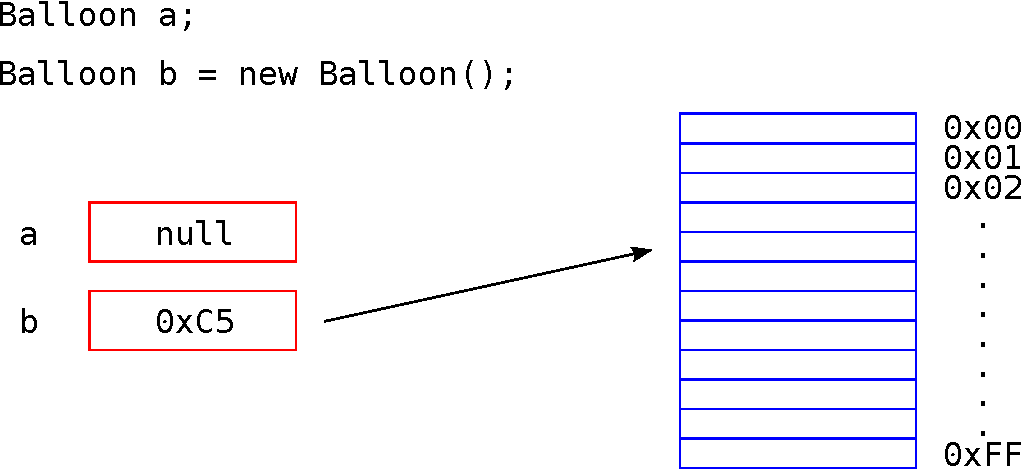
\includegraphics[width=0.5\textwidth]{null.pdf}
	\caption{A declared and initialized object in comparison.}
	\label{fig:null}
\end{figure}

\subsubsection{Chapter 4.15 to 4.17 - Summary}

\subsubsection*{Exercise 19}
\textit{Solve the exercises 4.62 to 4.65}\\

\textbf{4.62} \lstinline{Person[] people;}

\textbf{4.63} \lstinline{boolean[] vacant;}

\textbf{4.64} ???

\textbf{4.65} The declaration is wrong (syntax). It should look like

\lstinline{int[] counts;}

\lstinline{boolean[] occupied = new boolean[5000];}

\subsubsection*{Exercise 20}
\textit{Solve the exercises 4.66 to 4.68}\\

\textbf{4.66}
\begin{lstlisting}
double[] readings;
String[] urls;
TicketMachine[] machines;

readings = new double[6];
urls = new String[90];
machines = new TicketMachine[5];
\end{lstlisting}

\textbf{4.67} With \lstinline{String[] labels = new String[20]} 20 String 
objects are created.

\textbf{4.68} The correct expression is 
\lstinline{double[] piece = new double[50];}

\subsubsection*{Exercise 21}
\textit{What are the pros and cons of Arrays?}\\

\begin{itemize}
	\item[\ding{51}] Arrays are more efficient in access.
	\item[\ding{51}] Arrays can store primitive-types as well as objects.
	\item[\ding{55}] Arrays have a fixed size. 
\end{itemize}

\subsubsection*{Exercise 22}
\textit{How do you get the length of an Array?}\\

The length of an array is accessable by the \lstinline{length} operator.

\begin{lstlisting}
// create an array of type int with the length 50
int[] i = new int[50];

// return the length of the array
public int getLength(int[] array)
{
	return array.length;
}
\end{lstlisting}

\subsubsection*{Exercise 23}
\textit{Solve the exercises 4.69, 4.71, 4.73 and 4.74}\\

\textbf{4.69}
This will fail in an error called \textit{Out Of Bound Execption}.

\textbf{4.71}

\begin{lstlisting}
public void printGreater(double[] marks, double mean)
{
	for(index = 0; index < marks.length;  index++)
	{
		if(marks[index] > mean)
		{
			System.out.println(marks[index])
		}
	}
}
\end{lstlisting}

\textbf{4.73}

\begin{lstlisting}
public int numberOfAccesses()
{
	int total = 0;
	for(ctr = 0; ctr < hourCounts.length; ctr++)
	{
		total += hourCounts[ctr]; 
	}
	return total;
}
\end{lstlisting}

\textbf{4.74}
